\hypertarget{the-method-of-moderation}{}
\subsection{The Method of Moderation}\label{sec:method-of-moderation}

  Unfortunately, this endogenous gridpoints solution is not very
  well-behaved outside the original range of gridpoints targeted by
  the solution method.  (Though other common solution methods are no
  better outside their own predefined ranges).
  Figure~\ref{fig:ExtrapProblem} demonstrates the point by plotting
  the amount of precautionary saving implied by a linear extrapolation
  of our approximated consumption rule (the consumption of the perfect
  foresight consumer $\cFuncAbove_{\prdt-1}$ minus our approximation to
  optimal consumption under uncertainty, $\Aprx{\cFunc}_{\prdt-1}$).
  Although theory proves that precautionary saving is always positive,
  the linearly extrapolated numerical approximation eventually
  predicts negative precautionary saving (at the point in the figure
  where the extrapolated locus crosses the horizontal axis).

  \hypertarget{ExtrapProblemPlot}{}
  \begin{figure}
    \includegraphics[width=6in]{./Figures/ExtrapProblemPlot}
    \caption{For Large Enough $m_{\prdt-1}$, Predicted Precautionary Saving is Negative (Oops!)}
    \label{fig:ExtrapProblem}
  \end{figure}

  This error cannot be fixed by extending the upper gridpoint; in the presence of serious uncertainty, the consumption rule will need to be evaluated outside of \textit{any} prespecified grid (because starting from the top gridpoint, a large enough realization of the uncertain variable will push next period's realization of assets above that top; a similar argument applies below the bottom gridpoint).  While a judicious extrapolation technique can prevent this problem from being fatal (for example by carefully excluding negative precautionary saving), the problem is often dealt with using inelegant methods whose implications for the accuracy of the solution are difficult to gauge.


%\renewcommand{\prdt}{t} % For the rest of the doc, use generic t vs t+1

  As a preliminary to our solution, define $\hNrm_{\Cntn}$ as end-of-period human wealth (the present discounted value of future labor income) for a perfect foresight version of the problem of a `risk optimist:' a period-$t$ consumer who believes with perfect confidence that the shocks will always take their expected value of \PermShkOn{1, $\tranShkEmp_{\prdt+n} = \Ex[\tranShkEmp]=1~\forall~n>0$ and $\permShk_{\prdt+n} = \Ex[\permShk]=1~\forall~n>0$.}  {1, $\tranShkEmp_{\prdt+n} = \Ex[\tranShkEmp]=1~\forall~n>0$.}  The solution to a perfect foresight problem of this kind takes the form\footnote{For a derivation, see \cite{BufferStockTheory}; $\MPCmin_{\prdt}$ is defined therein as the MPC of the perfect foresight consumer with horizon $\trmT-t$.}
  \begin{equation}\begin{gathered}\begin{aligned}
        \cFuncAbove_{\prdt}(\mNrm_{\prdt})  & = (\mNrm_{\prdt} + \hNrm_{\Cntn})\MPCmin_{\prdt} \label{eq:cFuncAbove}
        %
        \UnifiedNote{[no direct counterpart] (computational: upper-bound perfect foresight consumption rule for MoM)}
      \end{aligned}\end{gathered}\end{equation}
  for a constant minimal marginal propensity to consume $\MPCmin_{\prdt}$ given below.

  We similarly define $\hEndMin_{\Cntn}$ as `minimal human wealth,' the
  present discounted value of labor income if the shocks were to take on
  their worst possible value in every future period \PermShkOn
  {$\tranShkEmp_{\prdt+n} = \tranShkEmpMin ~\forall~n>0$ and $\permShk_{\prdt+n} =
    \permShkMin ~\forall~n>0$} {$\tranShkEmp_{\prdt+n} = \tranShkEmpMin
    ~\forall~n>0$} (which we define as corresponding to the beliefs of a
  `pessimist').

  \ctw{}{We will call a `realist' the consumer who correctly perceives the true
    probabilities of the future risks and optimizes accordingly.}

  A first useful point is that, for the realist, a lower bound for the
  level of market resources is $\Min{m}_{\prdt} = -\hEndMin_{\Cntn}$, because
  if $m_{\prdt}$ equalled this value then there would be a positive finite
  chance (however small) of receiving \PermShkOn
  {$\tranShkEmp_{\prdt+n}=\tranShkEmpMin$ and $\permShk_{\prdt+n}=\permShkMin$}
  {$\tranShkEmp_{\prdt+n}=\tranShkEmpMin$}
  in
  every future period, which would require the consumer to set $c_{\prdt}$
  to zero in order to guarantee that the intertemporal budget constraint
  holds\ctw{.}{~(this is the multiperiod generalization of the discussion in
    section \ref{subsec:LiqConstrSelfImposed} explaining the derivation of the `natural borrowing constraint' for period $\trmT-1$,
    $\Min{a}_{\prdt-1}$).}  Since consumption of zero yields negative
  infinite utility, the solution to the realist consumer's problem is not well
  defined for values of $m_{\prdt} < \Min{m}_{\prdt}$, and the limiting
  value of the realist's $c_t$ is zero as $m_{\prdt} \downarrow \Min{m}_{\prdt}$.

  Given this result, it will be convenient to define `excess' market
  resources as the amount by which actual resources exceed the lower
  bound, and `excess' human wealth as the amount by which mean expected human wealth
  exceeds guaranteed minimum human wealth:
  \begin{equation*}\begin{gathered}\begin{aligned}
        \aboveMin \mNrm_{\prdt}  & = m_{\prdt}+\overbrace{\hEndMin_{\Cntn}}^{=-\Min{m}_{\prdt}}
        \\  \aboveMin \hNrm_{\Cntn}  & = \hNrm_{\Cntn}-\hEndMin_{\Cntn}.
      \end{aligned}\end{gathered}\end{equation*}

  We can now transparently define the optimal
  consumption rules for the two perfect foresight problems, those of the
  `optimist' and the `pessimist.'  The `pessimist' perceives human
  wealth to be equal to its minimum feasible value $\hEndMin_{\Cntn}$ with certainty, so
  consumption is given by the perfect foresight solution
  \begin{equation*}\begin{gathered}\begin{aligned}
        \cFuncBelow_{\prdt}(m_{\prdt})  & = (m_{\prdt}+\hEndMin_{\Cntn})\MPCmin_{\prdt}
        \\  & = \aboveMin \mNrm_{\prdt}\MPCmin_{\prdt}
        .
      \end{aligned}\end{gathered}\end{equation*}

  The `optimist,' on the other hand, pretends that there is no uncertainty
  about future income, and therefore consumes
  \begin{equation*}\begin{gathered}\begin{aligned}
        \cFuncAbove_{\prdt}(m_{\prdt})  & = (m_{\prdt} +\hEndMin_{\Cntn} - \hEndMin_{\Cntn} + \hNrm_{\Cntn} )\MPCmin_{\prdt}
        \\    & = (\aboveMin \mNrm_{\prdt} + \aboveMin \hNrm_{\Cntn})\MPCmin_{\prdt}
        \\      & = \cFuncBelow_{\prdt}(m_{\prdt})+\aboveMin \hNrm_{\Cntn} \MPCmin_{\prdt}
        .
      \end{aligned}\end{gathered}\end{equation*}

  It seems obvious that the spending of the realist will be strictly greater
  than that of the pessimist and strictly less than that of the
  optimist.  Figure~\ref{fig:IntExpFOCInvPesReaOptNeedHiPlot} illustrates the proposition for the consumption rule in period $\trmT-1$.
  \hypertarget{IntExpFOCInvPesReaOptNeedHiPlot}{}
  \begin{figure}
    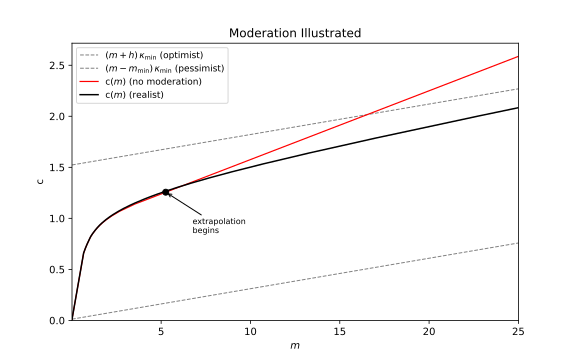
\includegraphics[width=6in]{./Figures/IntExpFOCInvPesReaOptNeedHiPlot}
    \caption{Moderation Illustrated: $\Min{\cFunc}_{\prdt-1} < \Aprx{\cFunc}_{\prdt-1} < \bar{\cFunc}_{\prdt-1}$}
    \label{fig:IntExpFOCInvPesReaOptNeedHiPlot}
  \end{figure}

  \indent The proof is more difficult than might be imagined, but
  the necessary work is done in \cite{BufferStockTheory} so we will take
  the proposition as a fact and proceed by manipulating the inequality:


  \begin{center}
    \begin{tabular}{rcl}
      $ \aboveMin \mNrm_{\prdt} \MPCmin_{\prdt} < $ & $ \cFunc_{\prdt}(\Min{m}_{\prdt}+\aboveMin \mNrm_{\prdt}) $ & $< (\aboveMin \mNrm_{\prdt}+\aboveMin \hNrm_{\Cntn})\MPCmin_{\prdt} $
      \\  $- \aboveMin \mNrm_{\prdt} \MPCmin_{\prdt} > $ & $ -\cFunc_{\prdt}(\Min{m}_{\prdt}+\aboveMin \mNrm_{\prdt}) $ & $> -(\aboveMin \mNrm_{\prdt}+\aboveMin \hNrm_{\Cntn})\MPCmin_{\prdt} $
      \\  $ \aboveMin \hNrm_{\Cntn} \MPCmin_{\prdt} > $ & $ \bar{\cFunc}_{\prdt}(\Min{m}_{\prdt}+\aboveMin \mNrm_{\prdt})-\cFunc_{\prdt}(\Min{m}_{\prdt}+\aboveMin \mNrm_{\prdt}) $ & $> 0$
      \\  $1 > $ & $ \underbrace{\left(\frac{\bar{\cFunc}_{\prdt}(\Min{m}_{\prdt}+\aboveMin \mNrm_{\prdt})-\cFunc_{\prdt}(\Min{m}_{\prdt}+\aboveMin \mNrm_{\prdt})}{\aboveMin \hNrm_{\Cntn} \MPCmin_{\prdt}}\right)}_{\equiv \Max{\koppa}_{\prdt}} $ & $> 0$
    \end{tabular}
  \end{center}

  \noindent  where the fraction in the middle of the last inequality is the ratio
  of actual precautionary saving (the numerator is the difference
  between perfect-foresight consumption and optimal consumption in the
  presence of uncertainty) to the maximum conceivable amount of
  precautionary saving (the amount that would be undertaken by the
  pessimist who consumes nothing out of any future income beyond the perfectly certain component).

  Defining $\mu_{\prdt} =
  \log \aboveMin \mNrm_{\prdt}$ (which can range from $-\infty$ to $\infty$), the object in the middle of the last inequality is
  \begin{equation}\begin{gathered}\begin{aligned}
        \Max{\koppa}_{\prdt}(\mu_{\prdt})   & \equiv  \left(\frac{\bar{\cFunc}_{\prdt}(\Min{m}_{\prdt}+e^{\mu_{\prdt}})-\cFunc_{\prdt}(\Min{m}_{\prdt}+e^{\mu_{\prdt}})}{\aboveMin \hNrm_{\Cntn} \MPCmin_{\prdt}}\right), \label{eq:koppa}
        %
        \UnifiedNote{[no direct counterpart] (computational: koppa — bounded interpolant between pessimist/optimist consumption)}
      \end{aligned}\end{gathered}\end{equation}
  and we now define
  \begin{equation}\begin{gathered}\begin{aligned}
        \Max{\chiFunc}_{\prdt}(\mu_{\prdt})  & = \log \left(\frac{1-\Max{\koppa}_{\prdt}(\mu_{\prdt})}{\Max{\koppa}_{\prdt}(\mu_{\prdt})}\right)
        \\  & = \log \left(1/\Max{\koppa}_{\prdt}(\mu_{\prdt})-1\right) \label{eq:chi}
        %
        \UnifiedNote{[no direct counterpart] (computational: chi — log-odds transform of koppa for interpolation)}
      \end{aligned}\end{gathered}\end{equation}
  which has the virtue that it is linear in the limit as $\mu_{\prdt}$ approaches $+\infty$.

  Given $\Max{\chiFunc}$, the consumption function can be recovered from
  \begin{equation}\begin{gathered}\begin{aligned}
        \Max{\cFunc}_{\prdt}  & = \bar{\cFunc}_{\prdt}-\overbrace{\left(\frac{1}{1+\exp(\Max{\chiFunc}_{\prdt})}\right)}^{=\Max{\koppa}_{\prdt}} \aboveMin \hNrm_{\Cntn} \MPCmin_{\prdt}. \label{eq:cFuncHi}
        %
        \UnifiedNote{𝒱.cFunc (partial: computational approximation of consumption policy via MoM)}
      \end{aligned}\end{gathered}\end{equation}

  Thus, the procedure is to calculate $\Max{\chiFunc}_{\prdt}$ at the points
  $\vctr{\mu}_{\prdt}$ corresponding to the log of the $\aboveMin
  \vctr{m}_{\prdt}$ points defined above, and then using these to construct an
  interpolating approximation $\Aprx{\Max{\chiFunc}}_{\prdt}$ from which we indirectly obtain our
  approximated consumption rule $\Aprx{\Max{\cFunc}}_{\prdt}$ by substituting $\Aprx{\Max{\chiFunc}}_{\prdt}$ for $\Max{\chiFunc}$ in equation \eqref{eq:cFuncHi}.

  Because this method relies upon the fact that the problem is easy to
  solve if the decision maker has unreasonable views (either in the
  optimistic or the pessimistic direction), and because the correct
  solution is always between these immoderate extremes, we call our
  solution procedure the `method of moderation.'

  Results are shown in Figure~\ref{fig:ExtrapProblemSolved}; a reader
  with very good eyesight might be able to detect the barest hint of a
  discrepancy between the Truth and the Approximation at the far
  righthand edge of the figure\ctw{.}{ -- a stark contrast with the calamitous
    divergence evident in Figure~\ref{fig:ExtrapProblem}.}{}
  \hypertarget{ExtrapProblemSolvedPlot}{}
  \begin{figure}
    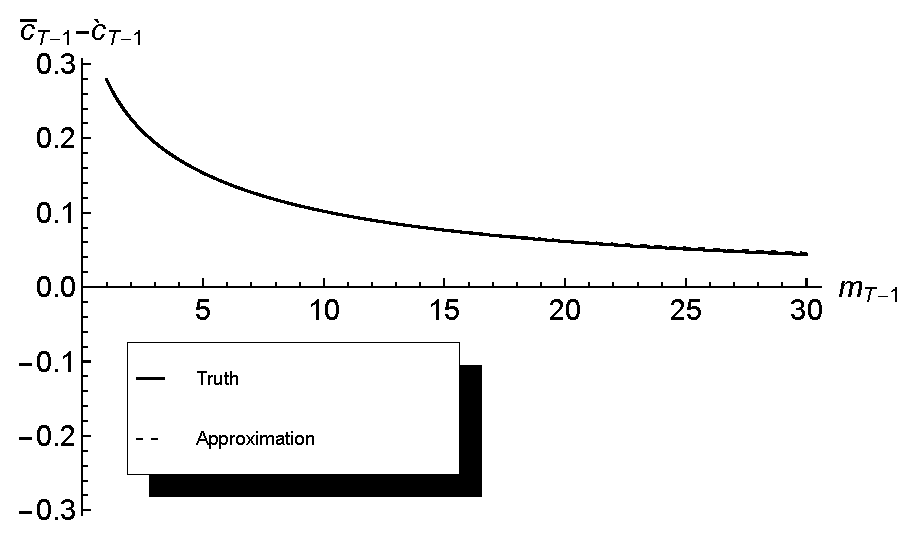
\includegraphics[width=6in]{./Figures/ExtrapProblemSolvedPlot}
    \caption{Extrapolated $\Aprx{\Max{\cFunc}}_{\prdt-1}$ Constructed Using the Method of Moderation}
    \label{fig:ExtrapProblemSolved}
  \end{figure}

\hypertarget{approximating-the-slope-too}{}
\subsection{Approximating the Slope Too}


Until now, we have calculated the level of consumption at various different gridpoints and used linear interpolation\ctw{.}{ (either directly for $\cFunc_{\prdt-1}$ or indirectly for, say, $\Max{\chiFunc}_{\prdt-1}$).}  But the resulting piecewise linear approximations have the unattractive feature that they are not differentiable at the `kink points' that correspond to the gridpoints where the slope of the function changes discretely.



\cite{BufferStockTheory} proves that the true consumption function for
this problem
is `smooth:' It
exhibits a well-defined unique marginal propensity to consume at every
positive value of $m$.  This suggests that we should calculate, not
just the level of consumption, but also the marginal propensity to
consume (henceforth $\MPC$) at each gridpoint, and then find an
interpolating approximation that smoothly matches both the level and the slope
at those points.

This requires us to differentiate \eqref{eq:koppa} and \eqref{eq:chi}, yielding
\begin{equation}\begin{gathered}\begin{aligned}
      \Max{\koppa}_{\prdt}^{\mu}(\mu_{\prdt})   & = (\aboveMin \hNrm_{\Cntn} \MPCmin_{\prdt})^{-1}e^{\mu_{\prdt}}\left(\MPCmin_{\prdt}-\overbrace{\cFunc^{\dm}_{\prdt}(\Min{m}_{\prdt}+e^{\mu_{\prdt}})}^{\equiv \MPCFunc_{\prdt}(\mNrm_{\prdt})}\right)  \label{eq:koppaPrime}
      \\ \Max{\chiFunc}_{\prdt}^{\mu}(\mu_{\prdt})  & = \left(\frac{-\Max{\koppa}_{\prdt}^{\mu}(\mu_{\prdt})/\Max{\koppa}_{\prdt}^{2}}{1/\Max{\koppa}_{\prdt}(\mu_{\prdt})-1}\right)
      %
      \UnifiedNote{[no direct counterpart] (computational: derivatives of koppa and chi for Hermite interpolation)}
    \end{aligned}\end{gathered}\end{equation}
and (dropping arguments) with some algebra these can be combined to yield
\begin{equation}\begin{gathered}\begin{aligned}
      \Max{\chiFunc}_{\prdt}^{\mu}  & = \left(\frac{\MPCmin_{\prdt} \aboveMin \mNrm_{\prdt} \aboveMin \hNrm_{\Cntn} (\MPCmin_{\prdt}-\MPC_{\prdt})}
        {(\cFuncAbove_{\prdt}-\cFunc_{\prdt})(\cFuncAbove_{\prdt}-\cFunc_{\prdt} - \MPCmin_{\prdt} \aboveMin \hNrm_{\Cntn})}\right).
      %
      \UnifiedNote{[no direct counterpart] (computational: combined derivative of chi for slope matching)}
    \end{aligned}\end{gathered}\end{equation}

To compute the vector of values of \eqref{eq:koppaPrime} corresponding
to the points in $\vctr{\mu}_{\prdt}$, we need the marginal propensities to
consume (designated $\MPC$) at each of the gridpoints,
$\cFunc^{\dm}_{\prdt}$ (the vector of such values is
$\vctr{\MPC}_{\prdt}$).  These can be obtained by differentiating the
Euler equation \eqref{eq:upEqbetaOp} (where we define
$\mFunc_{\Cntn}(a) \equiv \cFunc_{\Cntn}(a)+{a}$, and drop the (a) arguments to reduce clutter):
\begin{equation}\begin{gathered}\begin{aligned}
      \uFunc^{c}(\cFunc_{\Cntn})   & = \hat{\vFunc}_{\Cntn}^{\partial}(\mFunc_{\Cntn}-\cFunc_{\Cntn}),
      %
      \UnifiedNote{FOC of 𝒱: u'(c) = ℰ^{\partial}(a) (differentiated Euler equation for MPC computation)}
    \end{aligned}\end{gathered}\end{equation}
yielding a marginal propensity to
\textit{have consumed} $\cFunc_{\Cntn}^{\partial}$ at each gridpoint:
\begin{equation}\begin{gathered}\begin{aligned}
      \uPP(\cCntn)\cCntn^{\partial}  & = \hat{\vFunc}_{\Cntn}^{\partial\,\partial}(\mFunc_{\Cntn}-\cFunc_{\Cntn})
      \\ \cCntn^{\partial}  & = \hat{\vFunc}_{\Cntn}^{\partial\,\partial}(\mFunc_{\Cntn}-\cFunc_{\Cntn})/\uPP(\cCntn)
      %
      \UnifiedNote{[no direct counterpart] (computational: marginal propensity to have consumed from differentiated FOC)}
    \end{aligned}\end{gathered}\end{equation}
and the marginal propensity to consume at the beginning of the period is obtained from the marginal propensity to have consumed by differentiating the identity with respect to $\aNrm$:
\begin{equation*}\begin{gathered}\begin{aligned}
      \cCntn  & = \mFunc_{\Cntn} - \aNrm
      \\ \cCntn^{\partial}+1  & = \mFunc_{\Cntn}^{\partial}
    \end{aligned}\end{gathered}\end{equation*}
which, together with the chain rule $\cCntn^{\partial}  = \cFunc^{\dm}_{\Dcsn}\mFunc_{\Cntn}^{\partial}$, yields the MPC from
\begin{equation}\begin{gathered}\begin{aligned}
      \cFunc^{\dm}(\overbrace{\cCntn^{\partial}+1}^{=\mFunc_{\Cntn}^{\partial}})  & = \cCntn^{\partial}
      \\ \cFunc^{\dm}  & = \cCntn^{\partial}/(1+\cCntn^{\partial}) \label{eq:MPCfromMPTHC}.
      %
      \UnifiedNote{[no direct counterpart] (computational: MPC at gridpoints from marginal propensity to have consumed)}
    \end{aligned}\end{gathered}\end{equation}


Designating $\Aprx{\Max{\cFunc}}_{\prdt-1}$ as the approximated consumption rule obtained using an interpolating polynomial approximation to $\Max{\chiFunc}$ that matches both the level and the first derivative at the gridpoints, Figure~\ref{fig:IntExpFOCInvPesReaOptGapPlot} plots the difference between this latest approximation and the true consumption rule for period $\trmT-1$ up to the same large value (far beyond the largest gridpoint) used in prior figures.  Of course, at the gridpoints the approximation will exactly match the true function; but this figure illustrates that the approximation is quite accurate far beyond the last gridpoint (which is the last point at which the difference touches the horizontal axis).  (We plot here the difference between the two functions rather than the level plotted in previous figures, because in levels the difference between the approximate and the exact function would not be detectable even to the most eagle-eyed reader.)



\hypertarget{IntExpFOCInvPesReaOptGapPlot}{}
\begin{figure}
  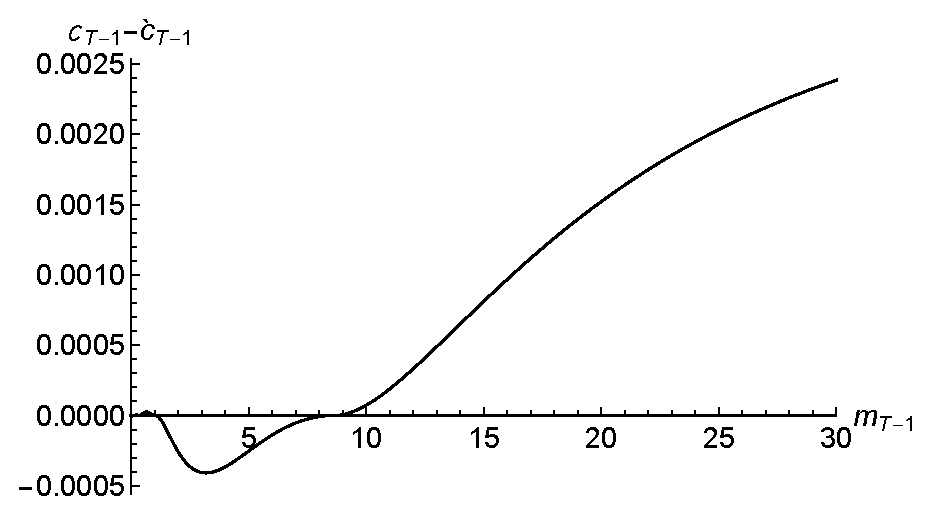
\includegraphics[width=6in]{./Figures/IntExpFOCInvPesReaOptGapPlot}
  \caption{Difference Between True $\cFunc_{\prdt-1}$ and $\Aprx{\Max{\cFunc}}_{\prdt-1}$ Is Minuscule}
  \label{fig:IntExpFOCInvPesReaOptGapPlot}
\end{figure}




\hypertarget{value}{}
\subsection{Value}


  Often it is useful to know the value function as well as the consumption rule.  Fortunately, many of the tricks used when solving for the consumption rule have a direct analogue in approximation of the value function.

  Consider the perfect foresight (or ``optimist's'') problem in period $\trmT-1$.  Using the fact that in a perfect foresight model the growth factor for consumption is $(\Rfree \DiscFac)^{1/\CRRA}$, we can use the fact that $\cNrm_{\prdt} = (\Rfree \DiscFac)^{1/\CRRA} \cNrm_{\prdt-1}$ to calculate the value function in period $\trmT-1$:
  \begin{equation*}\begin{gathered}\begin{aligned}
        \bar{\vFunc}_{\dcsn(\prdt-1)}(m_{\prdt-1})  & \equiv  \uFunc(\cNrm_{\prdt-1})+\DiscFac \uFunc(\cNrm_{\prdt})
        \\  & = \uFunc(\cNrm_{\prdt-1})\left(1+\DiscFac ((\DiscFac\Rfree)^{1/\CRRA})^{1-\CRRA}\right)
        % \\  & = \uFunc(\cNrm_{\prdt-1})\left(1+\DiscFac (\DiscFac\Rfree)^{1/\CRRA-1}\right)
        \\  & = \uFunc(\cNrm_{\prdt-1})\left(1+(\DiscFac\Rfree)^{1/\CRRA}/\Rfree\right)
        \\  & = \uFunc(\cNrm_{\prdt-1})\underbrace{\mbox{PDV}_{\prdt}^{T}(\cNrm)/\cNrm_{\prdt-1}}_{\equiv \PDVCoverc_{\prdt-1}^{T}}
      \end{aligned}\end{gathered}\end{equation*}
  where $\PDVCoverc_{\prdt}^{T}=\mbox{PDV}_{\prdt}^{T}(\cNrm)$ is the present discounted value of consumption, normalized by current consumption. Using the fact demonstrated in \cite{BufferStockTheory} that $\PDVCoverc_{\prdt}=\MPC^{-1}_{\prdt}$, a similar function can be constructed recursively for earlier periods, yielding the general expression \hypertarget{vFuncPF}{}
  \begin{equation}\begin{gathered}\begin{aligned}
        \bar{\vFunc}_{\dcsn(\prdt)}(m_{\prdt})  & = \uFunc(\bar{\cNrm}_{\prdt})\PDVCoverc_{\prdt}^{T}\label{eq:vFuncPF}
        \\  & = \uFunc(\bar{c}_{\prdt}) \MPCmin_{\prdt}^{-1} % 20190820
        \\  & = \uFunc((\aboveMin \mNrm_{\prdt}+\aboveMin \hNrm_{\Cntn})\MPCmin_{\prdt}) \MPCmin_{\prdt}^{-1} % 20190820
        \\  & = \uFunc(\aboveMin \mNrm_{\prdt}+\aboveMin \hNrm_{\Cntn})\MPCmin_{\prdt}^{1-\CRRA} \MPCmin_{\prdt}^{-1} % 20190820
        \\  & = \uFunc(\aboveMin \mNrm_{\prdt}+\aboveMin \hNrm_{\Cntn})\MPCmin_{\prdt}^{-\CRRA}  % 20190820
        %
        \UnifiedNote{𝒱(xᵥ) (partial: upper-bound perfect foresight decision-value function for MoM)}
      \end{aligned}\end{gathered}\end{equation}

  This can be transformed as
  \begin{equation*}\begin{gathered}\begin{aligned}
        \bar{\vInv}_{\prdt}  & \equiv  \left((1-\CRRA)\bar{\vFunc}_{\dcsn(\prdt)}\right)^{1/(1-\CRRA)}
        \\  & = \cNrm_{\prdt}(\PDVCoverc_{\prdt}^{T})^{1/(1-\CRRA)}
        \\  & = (\aboveMin \mNrm_{\prdt}+\aboveMin \hNrm_{\Cntn})\MPCmin_{\prdt}^{-\CRRA/(1-\CRRA)}   % 20190820
      \end{aligned}\end{gathered}\end{equation*}
  \MPCMatch{with derivative
    \begin{equation*}\begin{gathered}\begin{aligned}
          \bar{\vInv}_{\prdt}^m  & = (\mathbb{C}_{\prdt}^{T})^{1/(1-\CRRA)}\MPCmin_{\prdt},
          \\  & = \MPCmin_{\prdt}^{-\CRRA/(1-\CRRA)} % 20190820
        \end{aligned}\end{gathered}\end{equation*}}{}
  and since $\PDVCoverc_{\prdt}^{T}$ is a constant while the consumption
  function is linear, $\bar{\vInv}_{\prdt}$ will also be linear.

  We apply the same transformation to the value function for the problem with uncertainty (the ``realist's'' problem)\MPCMatch{ and differentiate}:
  \begin{equation*}\begin{gathered}\begin{aligned}
        \bar{\vInv}_{\prdt}  & = \left((1-\CRRA)\bar{\vFunc}_{\dcsn(\prdt)}(m_{\prdt})\right)^{1/(1-\CRRA)}
        \MPCMatch{\\ \bar{\vInv}^{\dm}_{\prdt}  & = \left((1-\CRRA)\bar{\vFunc}_{\dcsn(\prdt)}(m_{\prdt})\right)^{-1+1/(1-\CRRA)}\bar{\vFunc}_{\dcsn(\prdt)}^{\dm}(m_{\prdt})}{}
      \end{aligned}\end{gathered}\end{equation*}
  and an excellent approximation to the value function can be obtained by
  calculating the values of $\bar{\vInv}$ at the same gridpoints used by the
  consumption function approximation, and interpolating among those points.

  However, as with the consumption approximation, we can do even better if we
  realize that the $\bar{\vInv}$ function for the optimist's problem is
  an upper bound for the ${\vInv}$ function in the presence of uncertainty, and the value function
  for the pessimist is a lower bound. Analogously to \eqref{eq:koppa}, define an upper-case
  \begin{equation}\begin{gathered}\begin{aligned}
        \hat{\Koppa}_{\prdt}(\mu_{\prdt})   & = \left(\frac{\bar{\vInv}_{\prdt}(\Min{m}_{\prdt}+e^{\mu_{\prdt}})-\vInv_{\prdt}(\Min{m}_{\prdt}+e^{\mu_{\prdt}})}{\aboveMin \hNrm_{\Cntn} \MPCmin_{\prdt} (\PDVCoverc_{\prdt}^{T})^{1/(1-\CRRA)}}\right) \label{eq:Koppa}
        %
        \UnifiedNote{[no direct counterpart] (computational: Koppa — bounded interpolant for inverted value function 𝒱)}
      \end{aligned}\end{gathered}\end{equation}
  \MPCMatch{with derivative (dropping arguments)
    \begin{equation}\begin{gathered}\begin{aligned}
          \hat{\Koppa}_{\prdt}^{\mu}   & = (\aboveMin \hNrm_{\Cntn} \MPCmin_{\prdt} (\PDVCoverc_{\prdt}^{T})^{1/(1-\CRRA)})^{-1}e^{\mu_{\prdt}}\left(\bar{\vInv}^{\dm}_{\prdt}-\vInv^{\dm}_{\prdt}\right) \label{eq:KoppaPrime}
          % \\  & =  (\aboveMin \hNrm_{\Cntn} \MPCmin_{\prdt})^{-1}e^{\mu_{\prdt}}\left((\PDVCoverc_{\prdt}^{T})^{1/(1-\CRRA)}\MPCmin_{\prdt}-\left((1-\CRRA)\vFunc_{\dcsn(\prdt)}(m_{\prdt})\right)^{-1+1/(1-\CRRA)}\vFunc_{\dcsn(\prdt)}^{m}(m_{\prdt})\right)  \notag
          %
          \UnifiedNote{[no direct counterpart] (computational: derivative of Koppa for Hermite interpolation of 𝒱)}
        \end{aligned}\end{gathered}\end{equation}}{}
  and an upper-case version of the $\chiFunc$ equation in \eqref{eq:chi}:
  \begin{equation}\begin{gathered}\begin{aligned}
        \hat{\Chi}_{\prdt}(\mu_{\prdt})  & = \log \left(\frac{1-\hat{\Koppa}_{\prdt}(\mu_{\prdt})}{\hat{\Koppa}_{\prdt}(\mu_{\prdt})}\right)
        \\  & = \log \left(1/\hat{\Koppa}_{\prdt}(\mu_{\prdt})-1\right) \label{eq:Chi}
        %
        \UnifiedNote{[no direct counterpart] (computational: Chi — log-odds transform of Koppa for value function interpolation)}
      \end{aligned}\end{gathered}\end{equation}
  \MPCMatch{with corresponding derivative
    \begin{equation}\begin{gathered}\begin{aligned}
          \hat{\Chi}_{\prdt}^{\mu}  & = \left(\frac{-\hat{\Koppa}_{\prdt}^{\mu}/\hat{\Koppa}_{\prdt}^{2}}{1/\hat{\Koppa}_{\prdt}-1}\right)
          %
          \UnifiedNote{[no direct counterpart] (computational: derivative of Chi for value function interpolation)}
        \end{aligned}\end{gathered}\end{equation}}{}
  and if we approximate these objects then invert them (as above with
  the $\Max{\koppa}$ and $\Max{\chiFunc}$ functions) we obtain a very high-quality
  approximation to our inverted value function at the same points for
  which we have our approximated value function:
  \begin{equation}\begin{gathered}\begin{aligned}
        \hat{\vInv}_{\prdt}  & = \bar{\vInv}_{\prdt}-\overbrace{\left(\frac{1}{1+\exp(\hat{\Chi}_{\prdt})}\right)}^{=\hat{\Koppa}_{\prdt}} \aboveMin \hNrm_{\Cntn} \MPCmin_{\prdt} (\PDVCoverc_{\prdt}^{T})^{1/(1-\CRRA) }
        %
        \UnifiedNote{𝒱(xᵥ) (partial: computational approximation of inverted decision-value function via MoM)}
      \end{aligned}\end{gathered}\end{equation}
  from which we obtain our approximation to the value function\MPCMatch{ and its derivatives~}~as \hypertarget{vHatFunc}{}
  \begin{equation}\begin{gathered}\begin{aligned}
        \hat{\vFunc}_{\dcsn(\prdt)}  & = \uFunc(\hat{\vInv}_{\prdt})
        \\  \hat{\vFunc}^{\dm}_{\dcsn(\prdt)}  & = \uFunc^{c}(\hat{\vInv}_{\prdt}) \hat{\vInv}^{\dm}
        \MPCMatch{\\  \hat{\vFunc}^{\dm\dm}_{\dcsn(\prdt)}  & = \uFunc^{cc}(\hat{\vInv}_{\prdt}) (\hat{\vInv}^{\dm})^{2} + \uFunc^{c}(\hat{\vInv}_{\prdt})\hat{\vInv}^{\dm\dm}}{}
        .
        %
        \UnifiedNote{𝒱(xᵥ), 𝒱^{\partial}(xᵥ) (partial: computational approximation of decision-value function and derivatives via MoM)}
      \end{aligned}\end{gathered}\end{equation}

  Although a linear interpolation that matches the level of $\vInv$ at the gridpoints is simple, a Hermite interpolation that matches both the level and the derivative of the $\bar{\vInv}_{\prdt}$ function at the gridpoints has the considerable virtue that the $\bar{\vFunc}_{\dcsn(\prdt)}$ derived from it numerically satisfies the envelope theorem at each of the gridpoints for which the problem has been solved.

  \MPCMatch{If we use the double-derivative calculated above to produce a higher-order Hermite polynomial, our approximation will also match
    marginal propensity to consume at the gridpoints; this would
    guarantee that the consumption function generated from the value
    function would match both the level of consumption and the
    marginal propensity to consume at the gridpoints; the numerical
    differences between the newly constructed consumption function and
    the highly accurate one constructed earlier would be negligible
    within the grid.}{}


\hypertarget{refinement-a-tighter-upper-bound}{}
\subsection{Refinement: A Tighter Upper Bound}
  \cite{BufferStockTheory} derives an upper limit  $\MPCmax_{\prdt}$ for the MPC as $m_{\prdt}$
  approaches its lower bound.  Using this
  fact plus the strict concavity of the consumption function yields the
  proposition that
  \begin{equation}\begin{gathered}\begin{aligned}
        \cFunc_{\prdt}(\Min{m}_{\prdt}+\aboveMin \mNrm_{\prdt}) & < \MPCmax_{\prdt} \aboveMin \mNrm_{\prdt}.
        %
        \UnifiedNote{[no direct counterpart] (computational: tighter upper bound on consumption using MPCmax)}
      \end{aligned}\end{gathered}\end{equation}

  The solution method described above does not guarantee that
  approximated consumption will respect this constraint between gridpoints, and a failure to
  respect the constraint can occasionally cause computational problems in solving
  or simulating the model.  Here, we
  describe a method for constructing an approximation that always
  satisfies the constraint.

  \begin{comment} % Old text needs to be revised or eliminated
    That is, the realist's consumption function is bounded from above by both
    the \textit{unconstrained} optimist's problem already treated, as well as
    by the \textit{constrained} optimist's problem, which is a 45 degree line
    originating from $\Min{m}_{\prdt}$ on the $m$-axis, as shown in
    Figure~\ref{fig:IntExpFOCInvPesReaOptNeed45Plot}. The same is true for
    the value function, as illustrated in Figure
    \ref{fig:IntExpFOCInvPesReaOptNeed45ValuePlot}.

    \hypertarget{IntExpFOCInvPesReaOptNeed45Plot}{}
    \begin{figure}
      \includegraphics[width=6in]{./Figures/IntExpFOCInvPesReaOptNeed45Plot}
      \caption{45 Degree Line as Another Upper Bound}
      \label{fig:IntExpFOCInvPesReaOptNeed45Plot}
    \end{figure}

    \hypertarget{IntExpFOCInvPesReaOptNeed45ValuePlot}{}
    \begin{figure}
      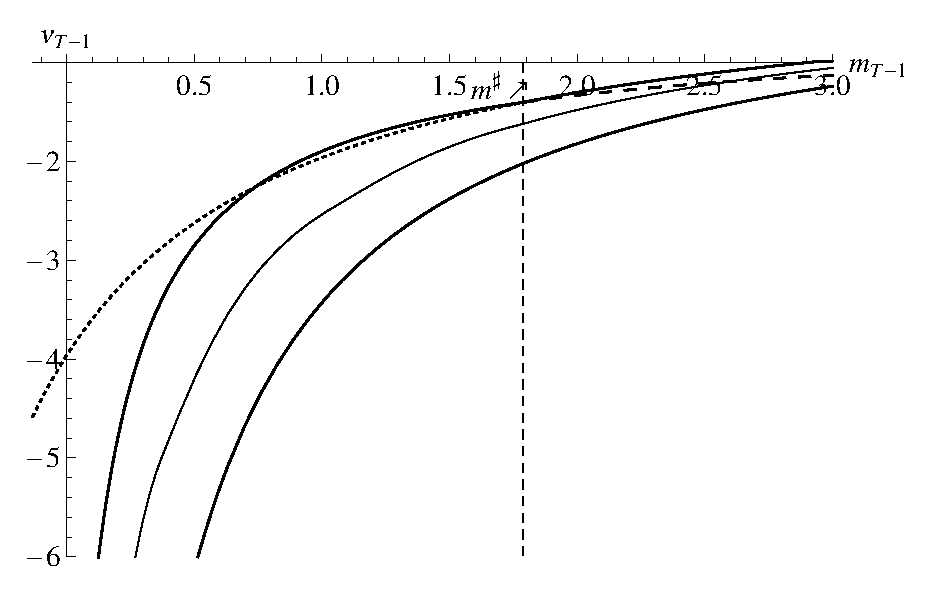
\includegraphics[width=6in]{./Figures/IntExpFOCInvPesReaOptNeed45ValuePlot}
      \caption{A Constrained Optimist's Value Function as Another Upper Bound}
      \label{fig:IntExpFOCInvPesReaOptNeed45ValuePlot}
    \end{figure}

  \end{comment}

  \newcommand{\mtCusp}{\ensuremath{\mNrm_{\prdt}^{\#}}}
  % \newcommand{\aboveMin \mtCusp}{\ensuremath{\aboveMin \mNrm_{\prdt}^{\#}}}

  Defining $\mtCusp$ as the `cusp' point where the two upper bounds
  intersect:
  \begin{equation*}\begin{gathered}\begin{aligned}
        \left(\aboveMin \mtCusp+\aboveMin \hNrm_{\Cntn}\right)\MPCmin_{\prdt}  & =  \MPCmax_{\prdt} \aboveMin \mtCusp \\
        \aboveMin \mtCusp  & =  \frac{\MPCmin_{\prdt}\aboveMin \hNrm_{\Cntn}}{(1-\MPCmin_{\prdt})\MPCmax_{\prdt}} \\
        \mtCusp  & =  \frac{\MPCmin_{\prdt}\hNrm_{\Cntn}-\hEndMin_{\Cntn}}{(1-\MPCmin_{\prdt})\MPCmax_{\prdt}},
      \end{aligned}\end{gathered}\end{equation*}
  we want to construct a consumption function for $m_{\prdt} \in (\Min{m}_{\prdt}, \mtCusp]$ that respects the
  tighter upper bound:
  \begin{center}
    \begin{tabular}{rcl}
      $ \aboveMin \mNrm_{\prdt} \MPCmin_{\prdt} < $ & $ \cFunc_{\prdt}(\Min{m}_{\prdt}+\aboveMin \mNrm_{\prdt}) $ & $< \MPCmax_{\prdt} \aboveMin \mNrm_{\prdt} $
      % \\  $-\aboveMin \mNrm_{\prdt} \MPCmin_{\prdt} > $ & $ -\cFunc_{\prdt}(\Min{m}_{\prdt}+\aboveMin \mNrm_{\prdt}) $ & $> -\aboveMin \mNrm_{\prdt} $
      \\  $ \aboveMin \mNrm_{\prdt}(\MPCmax_{\prdt}- \MPCmin_{\prdt}) > $ & $ \MPCmax_{\prdt} \aboveMin \mNrm_{\prdt}-\cFunc_{\prdt}(\Min{m}_{\prdt}+\aboveMin \mNrm_{\prdt}) $ & $> 0$
      \\  $1 > $ & $ \left(\frac{\MPCmax_{\prdt} \aboveMin \mNrm_{\prdt}-\cFunc_{\prdt}(\Min{m}_{\prdt}+\aboveMin \mNrm_{\prdt})}{\aboveMin \mNrm_{\prdt}(\MPCmax_{\prdt}- \MPCmin_{\prdt})}\right) $ & $> 0$.
    \end{tabular}
  \end{center}

  Again defining $\mu_{\prdt} =\log \aboveMin \mNrm_{\prdt}$, the object in the middle of the inequality is
  \begin{equation*}\begin{gathered}\begin{aligned}
        \Min{\koppa}_{\prdt}(\mu_{\prdt})  & \equiv  \frac{\MPCmax_{\prdt}-\cFunc_{\prdt}(\Min{m}_{\prdt}+e^{\mu_{\prdt}})e^{-\mu_{\prdt}}}{\MPCmax_{\prdt}-\MPCmin_{\prdt}} \label{eq:koppaL}
        \MPCMatch{\\ \Min{\koppa}^{\mu}_{\prdt}(\mu_{\prdt})  & = \frac{\cFunc_{\prdt}(\Min{m}_{\prdt}+e^{\mu_{\prdt}})e^{-\mu_{\prdt}}-\MPCFunc_{\prdt}^{\dm}(\Min{m}_{\prdt}+e^{\mu_{\prdt}})}{\MPCmax_{\prdt}-\MPCmin_{\prdt}}}{} .
      \end{aligned}\end{gathered}\end{equation*}

  As $m_{\prdt}$ approaches
  $-\Min{m}_{\prdt}$, $\Min{\koppa}_{\prdt}(\mu_{\prdt})$ converges to zero, while as $m_{\prdt}$
  approaches $+\infty$, $\Min{\koppa}_{\prdt}(\mu_{\prdt})$ approaches $1$.

  As before, we can derive an approximated consumption function; call it $\Aprx{\Min{\cFunc}}_{\prdt}$.  This function will clearly do a better job approximating the consumption function for low values of $\mNrm_{\prdt}$ while the previous approximation will perform better for high values of $\mNrm_{\prdt}$.

  For middling values of $\mNrm$ it is not clear which of these functions will perform better.  However, an alternative is available which performs well.  Define the highest gridpoint below $\mtCusp$ as $\bar{\check{\mNrm}}_{\prdt}^{\#}$ and the lowest gridpoint above $\mtCusp$ as $\Min{\hat{\mNrm}}_{\prdt}^{\#}$.  Then there will be a unique interpolating polynomial that matches the level and slope of the consumption function at these two points.  Call this function $\tilde{\cFunc}_{\prdt}(\mNrm)$.

  Using indicator functions that are zero everywhere except for specified intervals,
  \begin{equation*}\begin{gathered}\begin{aligned}
        \vctr{1}_{\text{Lo}}(\mNrm)  & = 1 \text{~if $          \mNrm \leq  \bar{\check{\mNrm}}_{\prdt}^{\#} \phantom{< \mNrm <   \Min{\hat{\mNrm}}_{\prdt}^{\#}          \leq \mNrm}$}
        \\  \vctr{1}_{\text{Mid}}(\mNrm)  & = 1 \text{~if $\phantom{ \mNrm \leq}~ \bar{\check{\mNrm}}_{\prdt}^{\#}          < \mNrm <   \Min{\hat{\mNrm}}_{\prdt}^{\#} \phantom{\leq \mNrm}$}
        \\  \vctr{1}_{\text{Hi}}(\mNrm)  & = 1 \text{~if $\phantom{ \mNrm \leq  ~\bar{\check{\mNrm}}_{\prdt}^{\#}          < \mNrm < } \Min{\hat{\mNrm}}_{\prdt}^{\#}           \leq \mNrm$}
      \end{aligned}\end{gathered}\end{equation*}
  we can define a well-behaved approximating consumption function
  \begin{equation}\begin{gathered}\begin{aligned}
        \Aprx{\cFunc}_{\prdt}  & = \vctr{1}_{\text{Lo}} \Aprx{\Min{\cFunc}}_{\prdt} + \vctr{1}_{\text{Mid}} \Aprx{\tilde{\cFunc}}_{\prdt}+\vctr{1}_{\text{Hi}} \Aprx{\Max{\cFunc}}_{\prdt}.
        %
        \UnifiedNote{[no direct counterpart] (computational: piecewise consumption approximation combining low/mid/high regions)}
      \end{aligned}\end{gathered}\end{equation}

  This just says that, for each interval, we use the approximation that
  is most appropriate.  The function is continuous and
  once-differentiable everywhere, and is therefore well behaved for
  computational purposes.
  \begin{comment}
    In practice, in our problem the difference due to this refinement is displayed in Figure \ref{fig:IntExpFOCInvPesReaOpt45GapPlot}.
    \hypertarget{IntExpFOCInvPesReaOpt45GapPlot}{}
    \begin{figure}
      \includegraphics[width=6in]{./Figures/IntExpFOCInvPesReaOpt45GapPlot}
      \caption{Difference Between $\Aprx{\Max{\cFunc}}_{L, T-1}$ and $\Aprx{\Max{\cFunc}}_{H,T-1}$ is Small}
      \label{fig:IntExpFOCInvPesReaOpt45GapPlot}
    \end{figure}
  \end{comment}

  We now construct an upper-bound value function implied for a consumer whose spending behavior is consistent with the refined upper-bound consumption rule.

  For $\mNrm_{\prdt} \geq \mNrm_{\prdt}^{\#}$, this consumption rule is the same as before,
  so the constructed upper-bound value function is also the same.  However, for
  values $\mNrm_{\prdt} < \mNrm_{\prdt}^{\#}$ matters are slightly more complicated.

  Start with the fact that at the cusp point,
  \begin{equation*}\begin{gathered}\begin{aligned}
        \bar{\vFunc}_{\dcsn(\prdt)}(\mtCusp)  & = \uFunc(\bar{\cNrm}_{\prdt}(\mtCusp))\PDVCoverc_{\prdt}^T \\
        & =  \uFunc(\aboveMin \mtCusp  \MPCmax_{\prdt})\PDVCoverc_{\prdt}^{T}
        .
      \end{aligned}\end{gathered}\end{equation*}

  But for \textit{all} $\mNrm_{\prdt}$,
  \begin{equation*}\begin{gathered}\begin{aligned}
        \bar{\vFunc}_{\dcsn(\prdt)}(\mNrm)  & = \uFunc(\bar{\cNrm}_{\prdt}(\mNrm))+ \bar{\vFunc}_{\EndPrd}(\mNrm-\bar{\cNrm}_{\prdt}(\mNrm)),
      \end{aligned}\end{gathered}\end{equation*}
  and we assume that for the consumer below the cusp point consumption is given by $\MPCmax \aboveMin \mNrm_{\prdt}$ so for $\mNrm_{\prdt}< \mtCusp$
  \begin{equation*}\begin{gathered}\begin{aligned}
        \bar{\vFunc}_{\dcsn(\prdt)}(\mNrm)  & = \uFunc( \MPCmax_{\prdt} \aboveMin \mNrm)+ \bar{\vFunc}_{\EndPrd}((1-\MPCmax_{\prdt})\aboveMin \mNrm),
      \end{aligned}\end{gathered}\end{equation*}
  which is easy to compute because $\bar{\vFunc}_{\EndPrd}(\aNrm_{\prdt}) = \DiscFac \bar{\vFunc}_{\dcsn(\prdt+1)}(\aNrm_{\prdt}\RNrmByG+1)$ where $\bar{\vFunc}_{\dcsn(\prdt)}$ is as defined above because a consumer who ends the current period with assets exceeding the lower bound will not expect to be constrained next period.  (Recall again that we are merely constructing an object that is guaranteed to be an \textit{upper bound} for the value that the `realist' consumer will experience.)  At the gridpoints defined by the solution of the consumption problem we can then construct
  \begin{equation*}\begin{gathered}\begin{aligned}
        \bar{\vInv}_{\prdt}(\mNrm)  & = ((1-\CRRA)\bar{\vFunc}_{\dcsn(\prdt)}(\mNrm))^{1/(1-\CRRA)}
      \end{aligned}\end{gathered}\end{equation*}
\MPCMatch{and its derivatives}{} which yields the appropriate vector for constructing $\check{\Chi}$ and $\check{\Koppa}$.  The rest of the procedure is analogous to that performed for the consumption rule and is thus omitted for brevity.


\hypertarget{extension-a-stochastic-interest-factor}{}
\subsection{Extension: A Stochastic Interest Factor}


Thus far we have assumed that the interest factor is constant at $\Rfree$.  Extending the
previous derivations to allow for a perfectly forecastable time-varying interest factor $\Rfree_{\prdt}$
would be trivial.  Allowing for a stochastic interest factor is less trivial.


The easiest case is where the interest factor is i.i.d.,
  \begin{equation}\begin{gathered}\begin{aligned}
        \log \Risky_{\prdt+n} & \sim \Nrml(\rfree + \eprem - \sigma^{2}_{\risky}/2,\sigma^{2}_{\risky}) ~\forall~n>0 \label{eq:distRisky}
        %
        \UnifiedNote{defines distribution of R̃ (risky return shock process, IID)}
      \end{aligned}\end{gathered}\end{equation}
where $\eprem$ is the risk premium and the $\sigma^{2}_{\risky}/2$ adjustment to the mean log return
guarantees that an increase in $\sigma^{2}_{\risky}$ constitutes a mean-preserving spread in the level of the return.

This case is reasonably straightforward because \cite{merton:restat} and \cite{samuelson:portfolio} showed
that for a consumer without labor income (or with perfectly forecastable labor income) the consumption
function is linear, with an infinite-horizon MPC\footnote{See \handoutC{CRRA-RateRisk} for a derivation.}
\begin{equation}\begin{gathered}\begin{aligned}
      \MPC  & = 1- \left(\DiscFac  \Ex_{\Arvl}[\Risky_{\prdt+1}^{1-\CRRA}]\right)^{1/\CRRA} \label{eq:MPCExact}
      %
      \UnifiedNote{portfolio FOC result: MPC under IID risky R̃ (Merton-Samuelson)}
    \end{aligned}\end{gathered}\end{equation}
and in this case the previous analysis applies once we substitute this MPC for the one that characterizes
the perfect foresight problem without rate-of-return risk.

The more realistic case where the interest factor has some serial correlation is more complex.  We consider
the simplest case that captures the main features of empirical interest rate dynamics: An AR(1) process.  Thus
the specification is
\begin{equation}\begin{gathered}\begin{aligned}
      \risky_{\prdt+1}-\risky  & = (\risky_{\prdt}-\risky) \gamma + \epsilon_{\prdt+1}
      %
      \UnifiedNote{defines shock process: AR(1) dynamics for log risky return r̃}
    \end{aligned}\end{gathered}\end{equation}
where $\risky$ is the long-run mean log interest factor, $0 < \gamma < 1$ is the AR(1) serial correlation
coefficient, and $\epsilon_{\prdt+1}$ is the stochastic shock.

The consumer's problem in this case now has two state variables, $\mNrm_{\prdt}$ and $\risky_{\prdt}$, and
is described by
\begin{equation}\begin{gathered}\begin{aligned}
      \vFunc_{\dcsn(\prdt)}(m_{\prdt},\risky_{\prdt})  & = \max_{c_{\prdt}} ~ \uFunc(c_{\prdt})+
      \Ex_{\Arvl}[{\DiscFac}_{\prdt+1}\PermGroFacAdjV{\vFunc}_{\dcsn(\prdt+1)}(m_{\prdt+1},\risky_{\prdt+1})] \label{vNormedRisky}
      \\         & \text{s.t.}   \nonumber \\
      a_{\prdt}    & = m_{\prdt}-c_{\prdt} \nonumber
      \\      \risky_{\prdt+1}-\risky  & = (\risky_{\prdt}-\risky)\gamma + \epsilon_{\prdt+1} \notag
      \\      \Risky_{\prdt+1}  & = \exp(\risky_{\prdt+1}) \notag
      \\      m_{\prdt+1}  & = \underbrace{\left(\Risky_{\prdt+1}/\PermGroFac_{\prdt+1}\right)}_{\equiv \RNrm_{\prdt+1}}a_{\prdt}+\tranShkEmp_{\prdt+1} \nonumber.
      %
      \UnifiedNote{𝒱(xᵥ) = max_c { u(c) + β𝔼[ℰ(xₑ)] } with xᵥ=(m,r̃) — Bellman equation with stochastic return}
    \end{aligned}\end{gathered}\end{equation}

% Kiichi: I will need you to read the literature and figure out how exactly we want to choose the Markov points and transition probabilities.
% When done, you will fill in the [how] text below.

We approximate the AR(1) process by a Markov transition matrix using standard techniques.  The stochastic interest factor is allowed to take
on 11 values centered around the steady-state value $\risky$.  Given this Markov transition matrix, \textit{conditional} on the Markov AR(1) state the consumption functions for the `optimist' and the `pessimist' will still be linear,
with identical MPC's that are computed numerically.  Given these MPC's, the (conditional) realist's consumption function can be computed for each Markov state, and the converged consumption rules constitute the solution contingent on the dynamics of the stochastic
interest rate process.

In principle, this refinement should be combined with the previous one;
further exposition of this combination is omitted here because no new
insights spring from the combination of the two techniques.



\hypertarget{imposing-artificial-borrowing-constraints}{}
\subsection{Imposing `Artificial' Borrowing Constraints}

Optimization problems often come with additional constraints that must
be satisfied.  Particularly common is an `artificial' liquidity constraint that
prevents the consumer's net worth from falling below some value, often
zero.\footnote{The word artificial is chosen only because of its clarity in distinguishing
  this from the case of the `natural' borrowing constraint examined above; no derogation is
  intended -- constraints of this kind certainly exist in the real world.}  The problem then becomes
\begin{equation*}\begin{gathered}\begin{aligned}
      \vFunc_{\dcsn(\prdt-1)}(m_{\prdt-1})  & = \max_{\cNrm_{\prdt-1}} ~~ \uFunc(c_{\prdt-1}) + \Ex_{\prdt-1} [\DiscFac \PermGroFacAdjV{\vFunc}_{\cntn(T)}(m_{\prdt})] \label{eq:ConstrArt}
      \\ & \mbox{s.t.}  \nonumber
      \\ a_{\prdt-1}  & = m_{\prdt-1} - c_{\prdt-1}
      \\ m_{\prdt}  & = \RNrmByG_{\prdt} a_{\prdt-1} + \tranShkEmp_{\prdt}
      \\ a_{\prdt-1} & \geq 0 .
    \end{aligned}\end{gathered}\end{equation*}


By definition, the constraint will bind if the unconstrained consumer
would choose a level of spending that would violate the constraint.
Here, that means that the constraint binds if the $c_{\prdt-1}$
that satisfies the unconstrained FOC
\begin{equation}\begin{gathered}\begin{aligned}
      c_{\prdt-1}^{-\CRRA}  & = \vFunc^{\partial}_{{\cntn}(\prdt-1)}(m_{\prdt-1}-c_{\prdt-1}) \label{eq:cUnc}
      %
      \UnifiedNote{FOC of 𝒱: u'(c) = ℰ^{\partial}(m−c) — unconstrained Euler equation}
    \end{aligned}\end{gathered}\end{equation}
is greater than $m_{\prdt-1}$.  Call $\grave{\cFunc}^{\ast}_{\prdt-1}$ the approximated function
returning the level of $c_{\prdt-1}$ that satisfies \eqref{eq:cUnc}.
Then the approximated constrained optimal consumption function will be
  \begin{equation}\begin{gathered}\begin{aligned}
        \grave{\cFunc}_{\prdt-1}(m_{\prdt-1})  & = \min[{m}_{\prdt-1},\grave{\cFunc}^{\ast}_{\prdt-1}(m_{\prdt-1})] \label{eq:LiqCons}.
        %
        \UnifiedNote{[no direct counterpart] (computational: consumption policy under artificial borrowing constraint)}
      \end{aligned}\end{gathered}\end{equation}


The introduction of the constraint also introduces a sharp
nonlinearity in all of the functions at the point where the constraint
begins to bind.  As a result, to get solutions that are anywhere close
to numerically accurate it is useful to augment the grid of values of
the state variable to include the exact value at which the constraint
ceases to bind.  Fortunately, this is easy to calculate.  We know that
when the constraint is binding the consumer is saving nothing, which
yields marginal value of $\vFunc^{\partial}_{{\cntn}(\prdt-1)}(0)$. Further, when the
constraint is binding, $c_{\prdt-1} = m_{\prdt-1}$.  Thus, the largest
value of consumption for which the constraint is binding will be the
point for which the marginal utility of consumption is exactly equal
to the (expected, discounted) marginal value of saving 0.  We know
this because the marginal utility of consumption is a downward-sloping \newcommand{\tinyAmount}{\epsilon}
function and so if the consumer were to consume $\tinyAmount$ more,
the marginal utility of that extra consumption would be \textit{below}
the (discounted, expected) marginal utility of saving, and thus the
consumer would engage in positive saving and the constraint would no
longer be binding.  Thus the level of $m_{\prdt-1}$ at which the
constraint stops binding is:\footnote{The logic here repeats an insight from \cite{deatonLiqConstr}.}
\begin{equation}\begin{gathered}\begin{aligned}
      \uFunc^{c}(m_{\prdt-1})  & = \vFunc^{\partial}_{{\cntn}(\prdt-1)}(0)  \nonumber \\
      m_{\prdt-1}  & = (\vFunc^{\partial}_{{\cntn}(\prdt-1)}(0))^{(-1/\CRRA)}  \nonumber
      \\        & = \cFunc_{{\cntn}(\prdt-1)}(0). \label{eq:LCbindsTm1}
      %
      \UnifiedNote{[no direct counterpart] (computational: m value where liquidity constraint ceases to bind)}
    \end{aligned}\end{gathered}\end{equation}

\hypertarget{cVScCon}{}
\begin{figure}
  \includegraphics[width=6in]{./Figures/cVScCon}
  \caption{Constrained (solid) and Unconstrained (dashed) Consumption}
  \label{fig:cVScCon}
\end{figure}

The constrained problem is solved in section ``Artificial Borrowing Constraint''
of the notebook, where the variable
\texttt{constrained} is set to be a boolean type object. If the value of \texttt{constrained}
is true, then the constraint is binding and their consumption behavior is computed to match
\eqref{eq:LiqCons}. The resulting consumption rule is shown in Figure \ref{fig:cVScCon}. For comparison purposes,
the approximate unconstrained consumption rule is
reproduced as the solid line; this is accomplished by setting the boolean value
of \texttt{constrained} to false.

The presence of the liquidity
constraint requires three changes to the procedures outlined above:
\begin{enumerate}
\item We redefine
  $\hEndMin_{\Cntn}$, which now is the PDV of receiving
  $\tranShkEmp_{\prdt+1}=\tranShkEmpMin$ next period and
  $\tranShkEmp_{\prdt+n}=0~\forall~n>1$ -- that is, the pessimist believes he
  will receive nothing beyond period $t+1$
\item We augment the end-of-period \code{aVec} with zero and with a point with a small positive value so that the generated
  {\mVec} will the binding point $\mNrm^{\#}$ and a point just above it (so that we can better capture the curvature
  around that point)
\item We redefine the optimal consumption rule as
  in equation (\ref{eq:LiqCons}).  This ensures that the
  liquidity-constrained `realist' will consume more than the redefined
  `pessimist,' so that we will have $\koppa$ still between $0$ and $1$
  and the `method of moderation' will proceed smoothly.
\end{enumerate}

As expected, the liquidity constraint only causes a divergence between the two functions at the point where the optimal unconstrained consumption rule runs into the 45 degree line.

\hypertarget{recursion}{}
\section{Recursion}\label{sec:recursion}

\hypertarget{theory}{}
\subsection{Theory}
Before we solve for periods earlier than $\trmT-1$, we assume for
convenience that in each such period a liquidity constraint exists of
the kind discussed above, preventing $c$ from exceeding $m$. This
simplifies things a bit because now we can always consider an
\code{aVec} that starts with zero as its smallest element.

Recall now equations~(\ref{eq:vEndPrimeTm1}) and (\ref{eq:upEqbetaOp}):
\begin{equation*}\begin{gathered}\begin{aligned}
      \vFunc^{\partial}_{\Cntn}(a_{\prdt})  & = \Ex_{\Arvl}[\DiscFac \Rfree \PermGroFac_{\prdt+1}^{-\CRRA}
      \uFunc^{c}(\cFunc_{\prdt+1}(\RNrmByG_{\prdt+1} a_{\prdt}+{\tranShkEmp}_{\prdt+1}))]
      \\\uFunc^{c}(c_{\prdt})   & = \vCntn^{\partial}(m_{\prdt}-c_{\prdt}).
    \end{aligned}\end{gathered}\end{equation*}
Assuming that the problem has been solved up to period $t+1$ (and thus assuming that we have an approximated $\Aprx{\cFunc}_{\prdt+1}(m_{\prdt+1})$), our solution method essentially involves using these two equations in succession to work back progressively from period $\trmT-1$ to the beginning of life.  Stated generally, the method is as follows.  (Here, we use the original, rather than the ``refined,'' method for constructing consumption functions; the generalization of the algorithm below to use the refined method presents no difficulties.)

\begin{enumerate}

\item For the grid of values $a_{\prdt,i}$ in \texttt{aVec\_eee}, numerically calculate the values
  of $\cFunc_{\Max{t}}(a_{\prdt,i})$ and $\cFunc_{\Max{t}}^{\partial}(a_{\prdt,i})$,
    \begin{equation}\begin{gathered}\begin{aligned}
          \cFunc_{\Max{t},i}  & = \left(\vCntn^{\partial}(a_{\prdt,i})\right)^{-1/\CRRA},
          \\                             & = \left(\DiscFac \Ex_{\Arvl} \left[\Rfree \PermGroFac_{\prdt+1}^{-\CRRA}(\grave{\cFunc}_{\prdt+1}(\RNrmByG_{\prdt+1} a_{\prdt,i} +      {\tranShkEmp}_{\prdt+1}))^{-\CRRA}\right]\right)^{-1/\CRRA}, \label{eq:vEndeq}
          \MPCMatch{\\        \cFunc^{\partial}_{\Max{t},i}  & = -(1/\CRRA)\left(\vCntn^{\partial}(a_{\prdt,i})\right)^{-1-1/\CRRA} \vCntn^{\partial\,\partial}(\aNrm_{\prdt,i}),}{}
          %
          \UnifiedNote{ℰ^{\partial}(xₑ) (partial: numerical computation of continuation-value derivative for EGM recursion)}
        \end{aligned}\end{gathered}\end{equation}
generating vectors of values $\vctr{\cFunc}_{\prdt}$\MPCMatch{ and $\vctr{\cFunc}^{\partial}_{\Max{t}}$.}{.}

\item Construct a corresponding vector of values of $\vctr{m}_{\prdt}=\vctr{\cNrm}_{\prdt}+\vctr{\aNrm}_{\prdt}$\MPCMatch{; similarly construct a corresponding list of MPC's $\vctr{\MPC}_{\prdt}$ using equation \eqref{eq:MPCfromMPTHC}.}{.}

\item Construct a corresponding vector $\vctr{\mu_{\prdt}}$, the levels\MPCMatch{ and first derivatives}{} of $\vctr{\koppa}_{\prdt}$, and the levels\MPCMatch{ and first derivatives}{} of $\vctr{\chi}_{\prdt}$.

\item Construct an interpolating approximation $\Aprx{\chi}_{\prdt}$ that\MPCMatch{ smoothly matches both the level and the slope}{the level} at those points.

\item If we are to approximate the value function, construct a corresponding list of values of $\vctr{v}_{\prdt}$, the levels\MPCMatch{ and first derivatives of $\vctr{\Koppa}_{\prdt}$,}{,} and the levels\MPCMatch{ and first derivatives}{} of $\hat{\vctr{\Chi}}_{\prdt}$; and construct an interpolating approximation function $\hat{\Chi}_{\prdt}$ that matches those points.
\end{enumerate}

With $\Aprx{\chi}_{\prdt}$ in hand, our approximate consumption function
is computed directly from the appropriate substitutions in \eqref{eq:cFuncHi}
and related equations.  With this consumption
rule in hand, we can continue the backwards recursion to period $t-1$
and so on back to the beginning of life.

Note that this loop does not contain an item for constructing $\hat{\vFunc}_{\dcsn(\prdt)}^{\partial}(m_{\prdt})$. This is because with $\Aprx{\Max{\cFunc}}_{\prdt}(m_{\prdt})$ in hand, we simply \textit{define} $\hat{\vFunc}^{\dm}_{\dcsn(\prdt)}(m_{\prdt}) = \uFunc^{c}(\Aprx{\Max{\cFunc}}_{\prdt}(m_{\prdt}))$ so there is no need to construct interpolating approximations - the function arises `free' (or nearly so) from our constructed $\Aprx{\Max{\cFunc}}_{\prdt}(m_{\prdt})$ via the usual envelope result (cf.\ \eqref{eq:envelope}).

